\section{Nanotecnologia}
La nanotecnología es un campo multidisciplinario que se centra en la manipulación y control de la materia a una escala extremadamente pequeña, específicamente en el rango de nanómetros, donde un nanómetro es igual a una mil millonésima parte de un metro \cite{nanotecnologia}. Este campo de estudio y aplicación busca comprender, diseñar y utilizar estructuras y dispositivos que operan a nivel nanométrico.

En esencia, la nanotecnología se enfoca en la capacidad de manipular la materia a nivel atómico y molecular para crear nuevos materiales con propiedades únicas y desarrollar dispositivos con funciones específicas. Esto incluye la fabricación y manipulación de nanopartículas, nanotubos, nanocompuestos y otras estructuras a escala nanométrica. La nanotecnología tiene aplicaciones en diversas áreas, como la medicina, la electrónica, la energía, la industria alimentaria, la construcción y muchas más, con el objetivo de mejorar el rendimiento y las características de los materiales y dispositivos a través de la innovación a nivel nanométrico.

    \begin{figure*}[h]
        \centering
        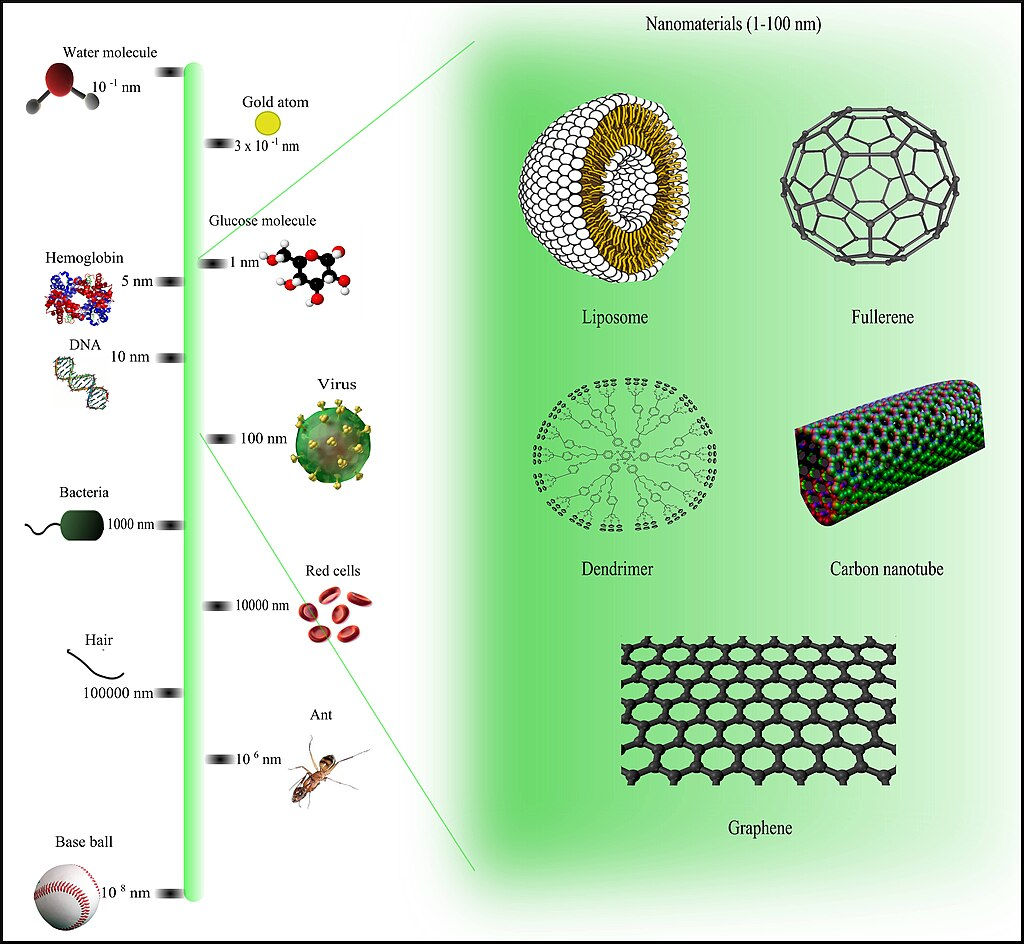
\includegraphics[height=7.8cm]{assets/figures/NAN.jpg}          
    \end{figure*}

\subsection{Materiales nanotecnologicos}
    \subsubsection{Nanopartículas}
    Partículas en el rango nanométrico, que pueden ser de diversos materiales como metales, cerámicas o polímeros. Una de sus caracteristicas es tener una gran relación área-superficie, lo que las hace ideales para aplicaciones como catalizadores, agentes de liberación controlada en medicina y filtros avanzados.
    \subsubsection{Nanotubos de Carbono}
    Estructuras cilíndricas compuestas completamente de carbono, con propiedades eléctricas y mecánicas excepcionales.Se utilizan en la fabricación de materiales compuestos avanzados, como el papel de nanotubos de carbono, y en aplicaciones electrónicas y biomédicas.
    \subsubsection{Grafeno}
    Una capa bidimensional de átomos de carbono dispuestos en una estructura hexagonal.Poseen alta conductividad eléctrica y térmica, y se utiliza en dispositivos electrónicos, baterías, sensores y materiales compuestos.
    \subsubsection{Nanocompuestos}
    Materiales que contienen nanopartículas o nanotubos dispersos en una matriz de otro material.Se caracterizan porque refuerzan las propiedades mecánicas, térmicas y eléctricas del material base, siendo empleados en la fabricación de polímeros reforzados y materiales compuestos avanzados.
    \subsubsection{Dendrímeros}
    Moléculas ramificadas con una estructura dendrítica, utilizadas en nanotecnología para la entrega controlada de fármacos y en la creación de nanoestructuras.
    \subsubsection{Nanocápsulas}
    Estructuras huecas a escala nanométrica utilizadas para encapsular y liberar moléculas específicas. Se aplican en la liberación controlada de medicamentos y en la protección de compuestos sensibles.
\subsection{Aplicaciones}
Los materiales nanotecnológicos tienen una amplia gama de aplicaciones en diversas industrias debido a sus propiedades únicas y a la capacidad de manipular la materia a escala nanométrica. Según \cite{castagnino-mat-nanotecnologia} algunas de las aplicaciones más destacadas de estos materiales:
    \begin{itemize}
        \item Imagen Médica: Agentes de contraste basados en nanomateriales para mejorar la calidad de imágenes médicas, como la resonancia magnética y la tomografía por emisión de positrones
        \item Nanotubos de Carbono y Grafeno: Aplicaciones en dispositivos electrónicos avanzados, como transistores y pantallas flexibles.
        \item Baterías y Almacenamiento de Energía: Uso de nanomateriales para mejorar la capacidad y velocidad de carga de baterías.
        \item Nanopartículas en Envases: Desarrollo de envases nanotecnológicos para prolongar la vida útil de los alimentos y monitorear su frescura.
        \item Nanosensores: Detección precisa de gases, compuestos químicos y biomarcadores para aplicaciones en salud y seguridad.
    \end{itemize}

    \begin{figure*}[h]
        \centering
        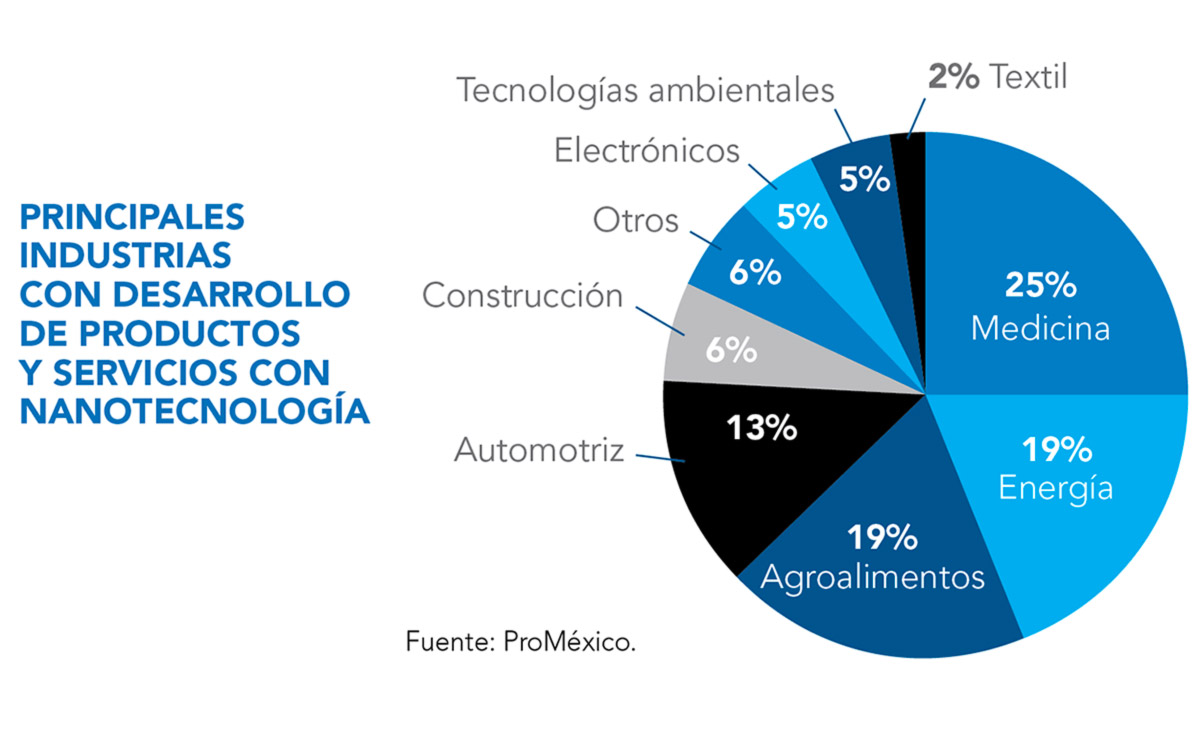
\includegraphics[height=7.8cm]{assets/figures/NANO.jpg}         
    \end{figure*}
